\documentclass{article}
\usepackage{tmlr}
% Uncomment for camera-ready: \usepackage[accepted]{tmlr}

\usepackage{amsmath, amssymb, amsthm}
\usepackage{booktabs}
\usepackage{microtype}
\usepackage{graphicx}
\usepackage{hyperref}
\usepackage{listings}
\usepackage{xcolor}

\lstset{
  basicstyle=\ttfamily\small,
  breaklines=true,
  frame=single,
  framesep=4pt,
  xleftmargin=8pt,
  xrightmargin=8pt,
  columns=fullflexible,
}

\newtheorem{theorem}{Theorem}
\newcommand{\deff}{d_{\mathrm{eff}}}

\title{Adaptive Width Growth from $d=2$:\\
A FLOP-Efficient Schedule for Snowman Language Models}

\author{\name{} Anonymous \\ \addr{} Anonymous}

\begin{document}
\maketitle

\begin{abstract}
We grow a 22-layer Snowman language model adaptively from $d{=}2$ on
FineWeb-Edu, using a math-derived schedule with no hand-tuned
thresholds (window-based progress test against the eval-batch noise
floor, entropy-based effective rank of the weight matrices, and a
divergence guard).  On a single RTX PRO 6000 Blackwell, the adaptive
run reaches validation cross-entropy $3.565$ at $d{=}496$ in $6.81$
wall-hours, using $1.0{\times}10^{18}$ FLOPs.  A fixed-$d{=}544$
end-to-end baseline trained from scratch with identical data,
tokenizer, optimizer, and learning rate, run for matched wall-clock
on the same GPU, reaches only $3.855$ at $1.66{\times}10^{18}$ FLOPs.
The adaptive run wins by $-0.29$ val CE and uses $\sim 1.7{\times}$
fewer FLOPs to its best.  We additionally report four supporting
contributions: (i) the asymmetric weight initialization that breaks
the dead-attention-head failure mode of zero-pad growth, (ii) a
$\sqrt{N}$ scaling argument $\eta_{\max} \sim \sigma_{\text{eval}} /
\sqrt{N}$ that explains why $\eta = 3{\times}10^{-4}$ destabilizes
training at small post-grow widths, (iii) a precision diagnostic
showing \texttt{bf16+AdamW8bit} introduces systematic optimizer-state
drift which \texttt{fp32 AdamW} removes at the same $\eta$, and (iv)
a stepped $d_{\text{head}}(d)$ schedule that keeps the number of
attention heads bounded ($\le 16$) and removes the linear-in-$d$
attention-memory term from the small-$d_{\text{head}}$ PAVING start.
\end{abstract}

\section{Introduction}

A central question in scaling language models is whether the FLOPs spent at
the final width are \emph{necessary} or simply \emph{spent}.  PAVING
\citep{paving} proves that, for a weight-tied $K$-block transformer trained
with per-depth local backprop, the relation between width and gradient
quality decouples: training at a small width $d_{\text{small}}$ accumulates
an honest, low-variance signal whose information content scales with
$\deff$ rather than with the eventual $d_{\max}$.

This decoupling motivates the obvious experiment --- start small, grow on
demand --- but the literature has not, to our knowledge, scaled it past toy
widths under a fixed FLOP budget.  We do.

\paragraph{Contributions.}
\begin{enumerate}
\item A \emph{math-derived} growth schedule.  A grow event fires only when
  three conjunctive conditions hold: (a) the per-FLOP information gain
  has fallen below the eval-batch noise floor, (b) the weight matrices'
  entropy-based effective rank is using most of the currently allocated
  dimensions, and (c) the current eval has not drifted above the running
  best by more than $2\sigma_{\text{eval}}$.  None of the thresholds is
  hand-tuned --- each is derived from the eval-noise distribution.
\item End-to-end run and a same-$d$ baseline.  The adaptive run with
  \texttt{fp32 AdamW} and stepped $d_{\text{head}}$ reaches val
  $3.565$ at $d{=}496$ in $6.81$ wall-hours on a single
  RTX PRO 6000 Blackwell.  At matched wall-clock $6.81$h on the same
  GPU, a fixed-$d{=}544$ E2E baseline trained from scratch with the
  same data stream, tokenizer, context length, optimizer, learning
  rate, and grad clip reaches only $3.855$.  Adaptive wins by $-0.29$
  val CE and also uses $\approx 1.7{\times}$ fewer FLOPs to reach its
  best ($1.0{\times}10^{18}$ vs $1.66{\times}10^{18}$).
\item A derivation of the dead-attention-head failure mode of pure zero-pad
  growth (Section~\ref{sec:asymmetric-init}) and the asymmetric weight
  initialization that breaks it: noise on the new rows of $W_q, W_k, W_v$,
  zero on the gates $W_o[:,\text{new cols}]$ and on the residual writers
  $\mathrm{ff}_2[\text{new rows},:]$, preserving the model's function while
  letting gradient flow into the new dimensions.
\end{enumerate}

We deliberately keep the framing modest.  Section~\ref{sec:ablations}
reports the same-$d$ E2E run that isolates the contribution of growth
from the contribution of $d{=}544$ itself.

\section{Theoretical Background}
\label{sec:theory}

The Snowman model is a transformer with a single weight-tied ``block''
applied $K$ times with per-step depth gates $\alpha_k$, trained with the
PAVING local backprop schedule.  We rely on three named results from
\citet{paving} and state them without proof; the proofs and a numerical
verification are at \href{https://doi.org/10.5281/zenodo.19454889}{Zenodo
DOI 10.5281/zenodo.19454889}.

\begin{theorem}[Width Detach, \citealt{paving} Thm.~13]
For a Snowman with hidden dim $d$ and $\deff < d$, the gradient of the local
loss restricted to the active subspace is $O(g^2)$ close to the full
gradient, where $g = \max_k \alpha_k$.
\end{theorem}

\begin{theorem}[Width Elasticity, \citealt{paving} Thm.~35]
\label{thm:elasticity}
Let $M_d$ be a Snowman with hidden dim $d$.  Define $M_{d'}$ for
$d' = d + n_{\text{new}} \cdot d_{\text{head}}$ by zero-padding all weights
and replacing every \texttt{LayerNorm} with \texttt{ActiveLayerNorm} whose
active set is $\{0, \ldots, d-1\}$.  Then $M_{d'}(x; K) = M_d(x; K)$ for all
inputs and all depths $K$.
\end{theorem}

\begin{theorem}[Per-FLOP Efficiency, \citealt{paving} Thm.~41]
The per-FLOP loss decrease at width $d$ is upper-bounded by
$O(\deff / d^2)$ when $d > \deff$.
\end{theorem}

Theorem~3 is an upper bound: it states the per-FLOP loss decrease at
width $d$ \emph{cannot exceed} $O(\deff / d^2)$ when $d > \deff$.  It
does not by itself guarantee that any optimizer achieves this rate.
The motivational reading is one-sided: at large $d$ with $d \gg
\deff$, the per-FLOP ceiling is low (so per-FLOP progress \emph{must}
be slow regardless of optimizer); at small $d$ just above $\deff$,
the per-FLOP ceiling is high (so there is room for progress, though
not guaranteed).  Our empirical contribution is the observation that,
under a standard AdamW optimizer and the trigger of \S\ref{sec:trigger},
the small-$d$ trajectories \emph{do} make progress close to the
ceiling --- which is what motivates growing $d$ on demand rather than
starting at the eventual target width.

\section{Method}
\label{sec:method}

\subsection{Architecture}
22-layer transformer, sinusoidal PE, weight-tied input/output
embedding.  $d_{\text{head}}$ is determined as a stepped function of
$d$ (\S\ref{sec:dhead}): $2$ at small $d$ to admit a valid head
decomposition from $d{=}2$, increasing as $d$ grows so that
$n_{\text{heads}} = d/d_{\text{head}}$ stays bounded.  LayerNorm is
replaced by ActiveLayerNorm (Theorem~\ref{thm:elasticity}) so that
mean/var are computed over the first $d_{\text{active}}$ dimensions
only.

\subsection{Adaptive Growth Trigger}
\label{sec:trigger}

Maximizing $\int dI/dt$ under FLOP budget $B$ gives a Lagrangian dual whose
KKT condition is ``per-FLOP info gain equal across all $d$ we visit''.
Operationally we cannot evaluate $dI/dt$ but can detect its drop below
noise, with one safety latch to avoid growing into a divergent state:

\begin{lstlisting}
W = 2000 steps         (~ 4 evals at EVAL_INTERVAL = 500)
sigma_eval ~ 0.05      (eval-batch CE std at EVAL_BATCHES = 20)
threshold = 2 * sigma_eval = 0.10

best_old = min(val_ce in [t-2W, t-W])
best_new = min(val_ce in [t-W,  t])
progress = best_old - best_new

stalled    <- progress < threshold
saturated  <- d_eff_W / d > 0.30           # mean over Wq,Wk,Wv,Wo,ff1,ff2
diverging  <- val_now - best_global > 2 * sigma_eval

if stalled and saturated and not in_recovery and not diverging:
    grow()
recovery_period = W
\end{lstlisting}

$\deff^W$ is the entropy-based effective rank of each block weight matrix,
averaged across blocks, normalized by $\min(\mathrm{shape})$.  Unlike
activation effective rank it has no positional-encoding contamination and
is essentially free to compute (six small SVDs per block per eval).

The three-way conjunction matters.  \emph{progress} alone fires whenever
validation drifts upward within noise, including divergent fluctuation past
$d \approx 70$; growing in that state only compounds the damage.  $\deff^W$
distinguishes ``model uses its current width'' from ``model has compressed
to a low-rank attractor''; only the former benefits from a grow.  The
divergence guard is the explicit safety latch: if the most recent eval is
already above the running best by more than $2\sigma_{\text{eval}}$, the
model is not on a plateau --- it is on a downward arc --- and we hold off
until it returns or sets a new best.

\subsection{Growth Operation}
\label{sec:asymmetric-init}

\begin{equation}
d_{\text{new}} \;=\; \mathrm{round}_{d_{\text{head}}(d_{\text{new}})}\!\Bigl(
\max\!\bigl(d + 2,\; \lceil d \cdot 1.05 / 2\rceil \cdot 2\bigr)\Bigr)
\end{equation}
where $\mathrm{round}_k$ rounds up to the nearest multiple of $k$ so
$d_{\text{new}}$ is divisible by the next-stage $d_{\text{head}}$
(\S\ref{sec:dhead}).  The base growth is multiplicative
($\times 1.05$, even-rounded) with an additive floor of $+2$ for
small $d$.

Naively zero-padding all weights at a grow event is exactly
function-preserving when combined with ActiveLayerNorm
(Theorem~\ref{thm:elasticity}), but it has a fatal interaction with the
attention head structure: the new head's rows of $W_q, W_k, W_v$ are zero,
hence its $q,k,v$ are zero, hence its head output is zero, hence its
contribution to the loss is zero, hence $\partial L / \partial W_q[\text{new
row},:] = 0$, and the new heads stay dead indefinitely.  Empirically, we
verified this by running a pure zero-pad variant: every weight matrix
after many grow events has numerical rank equal to the original $d$
(rank~2 for a run started at $d=2$), so adding more dimensions never adds
capacity.

We break the deadlock with an \emph{asymmetric} init.  For each grow, on
each block:
\begin{itemize}
\item $W_q, W_k, W_v$: the new \emph{rows} are filled with
  $10^{-3} \cdot \sigma_w \cdot \mathcal{N}(0,1)$ (small noise).  This makes
  $q, k, v$ at the new heads nonzero.
\item $W_o$: \emph{all} new entries (rows \emph{and} cols) stay at $0$.
\item $\mathrm{ff}_1$: new rows = small noise, new cols = $0$.
\item $\mathrm{ff}_2$: all new entries = $0$.
\end{itemize}
Because the writers to the residual stream ($W_o$ and $\mathrm{ff}_2$) are
still entirely zero at their new rows/cols, the model's output at the old
dimensions is unchanged (function approximately preserved, modulo the
one-time mean/var shift in ActiveLayerNorm when $d_{\text{active}}$ moves
from old to new).  But because the new attention heads now produce nonzero
$q,k,v$ and a nonzero attention output, the gates
$W_o[\text{old row},\text{new col}]$ start receiving real gradient,
$\partial L / \partial W_o[\text{old},\text{new}] = \text{err}_{h_{\text{old}}}
\cdot \text{attn\_out}_{\text{new col}} \neq 0$.  As the gates open, full
gradient flows back to $W_q,W_k,W_v[\text{new row},:]$ and the new heads
train normally.

This is the smallest perturbation we found that lifts pure zero-pad out of
its dead-head trap without introducing per-grow drift on the old dimensions.

\subsection{Training Details}
The main adaptive run uses \texttt{bf16} activations with the standard
\texttt{torch.optim.AdamW} (\texttt{fp32} optimizer state), at
$\mathrm{lr}=1.5{\times}10^{-4}$, $\mathrm{wd}=0.01$, grad-clip $1.0$,
with the stepped $d_{\text{head}}$ schedule of \S\ref{sec:dhead}.
FineWeb-Edu (\textsc{sample-10BT}) tokenized with the GPT-2 BPE into a
2.9B-token cache; first 2.899B for train, last 1M held out for eval.
Hardware: a single NVIDIA RTX PRO 6000 Blackwell (102 GB).

\subsection{Learning Rate Scaling}
\label{sec:lr-bound}

The value $\eta = 3{\times}10^{-4}$ is conventional for transformer
training \citep{adam}; we derive here a \emph{motivational scaling}
that explains why it is too large for the small-$d$ regime in which
a growing model spends most of its budget, and predicts the empirical
sweet spot $\eta_{\text{best}} \approx \mathrm{LR}/2$ that our main
run uses ($\eta = 1.5{\times}10^{-4}$, \S\ref{sec:results}).  The
inequality below is a Cauchy--Schwarz worst case, not a tight bound;
it correctly predicts the direction and order of magnitude but is
$\sim 20{\times}$ conservative in the constant, as the diagnostic in
Appendix~\ref{app:lr-sweep} documents.

In the AdamW steady state the per-coordinate update is approximately
$\Delta\theta_i \approx -\eta\cdot\mathrm{sign}(g_i)$, so the first-order
change of the loss after one step is
\begin{equation}
\Delta L \;\approx\; \nabla L^{\!\top} \!\Delta\theta
            \;=\; -\eta \sum_i |g_i|
            \;=\; -\eta\,\|g\|_1.
\end{equation}
By Cauchy--Schwarz, $\|g\|_1 \le \sqrt{N}\,\|g\|_2$, where $N$ is the number
of model parameters; combined with our gradient clip $\|g\|_2 \le 1$,
\begin{equation}
|\Delta L| \;\le\; \eta\,\sqrt{N}.
\end{equation}
For a window-based plateau test to function, single-step loss changes
should not exceed the eval-batch noise floor $\sigma_{\text{eval}}$
by much --- otherwise the trigger fires on optimization noise rather
than on saturation.  Equating the worst-case single-step bound to
$\sigma_{\text{eval}}$ gives a \emph{scaling}
\begin{equation}
\eta_{\max} \;\sim\; \frac{\sigma_{\text{eval}}}{\sqrt{N}}.
\label{eq:lr-bound}
\end{equation}
Two caveats.  First, the comparison of a single-step training
$\Delta L$ to a validation $\sigma_{\text{eval}}$ is an order-of-
magnitude argument, not a rigorous bound.  Second, the
Cauchy--Schwarz step $\|g\|_1 \le \sqrt{N} \|g\|_2$ is loose:
empirically $\|g\|_1 / \|g\|_2 \approx 86$ at $d{=}46$ while
$\sqrt{N} \approx 1700$, so Eq.~\ref{eq:lr-bound} is $\sim 20{\times}$
conservative in the constant (Appendix~\ref{app:lr-sweep}).  The
useful content is the $\sqrt{N}$ direction: as the model grows, the
admissible $\eta$ must shrink.

For our $d=46$ configuration with 22 layers (the post-grow state of
an early diagnostic run): $N \approx 3.2\times 10^{6}$ (the embedding
alone is $2.3{\times}10^6$ parameters), $\sigma_{\text{eval}} \approx
0.05$.  Eq.~\ref{eq:lr-bound} as written gives
$\eta_{\max} \approx 2.8\times 10^{-5}$, which is too conservative;
the empirical $\|g\|_1/\|g\|_2 \approx 86$ (vs $\sqrt{N} \approx
1700$) brings the admissible $\eta$ up to $\approx 6{\times}10^{-4}$.
The LR-sweep diagnostic at fixed $d{=}46$ (Appendix~\ref{app:lr-sweep})
identifies $\mathrm{LR}/2 = 1.5{\times}10^{-4}$ as the sweet spot
(best val $5.03$ at the end of the sweep window) and shows that
$\mathrm{LR}=3{\times}10^{-4}$ drifts upward, $\mathrm{LR}/3$ shows
occasional gradient spikes, and $\mathrm{LR}/30$ is too small to make
timely progress.  Our main run uses $\eta = 1.5{\times}10^{-4}$
throughout.

\subsection{Stepped $d_{\text{head}}$ schedule}
\label{sec:dhead}

PAVING starts at $d=2$, which requires $d_{\text{head}}=2$ at the
beginning (one head of dimension 2).  If $d_{\text{head}}$ is held
fixed at $2$ for the entire run, the number of attention heads grows
linearly with $d$, and the per-layer attention score tensor has shape
$B \times (d/2) \times T \times T$.  At $d=66$, $B=64$, $T=512$ this is
$2.2$ GB per layer in \texttt{fp32}; 22 layers retained for the
backward pass exceeds the GPU's 95 GB.

The fix is to step $d_{\text{head}}$ up with $d$:
\begin{equation}
d_{\text{head}}(d) \;=\;
\begin{cases}
2  & d \le 8 \\
4  & 8 < d \le 32 \\
8  & 32 < d \le 128 \\
16 & 128 < d \le 512 \\
32 & d > 512.
\end{cases}
\end{equation}
This bounds $n_{\text{heads}} = d / d_{\text{head}}$ above by $16$
throughout, so the per-layer attention tensor never exceeds
$B \times 16 \times T^2 \times \texttt{dtype}$ (here
$\approx 0.5$ GB in \texttt{fp32}, $0.25$ GB in \texttt{bf16}).

\paragraph{Transition mechanism.}  When a grow event crosses a
$d_{\text{head}}$ bracket, the new $d_{\text{new}}$ is rounded up to
the nearest multiple of the new $d_{\text{head}}$
(\S\ref{sec:asymmetric-init}) so that
$n_{\text{heads}}^{\text{new}} = d_{\text{new}} /
d_{\text{head}}^{\text{new}}$ is integer.  $W_q, W_k, W_v, W_o$ are
stored as $(d, d)$ Linears; the head decomposition is purely a
\texttt{view} for the per-head reshape inside the attention forward
pass.  When $d_{\text{head}}$ doubles, the stored weights do not
change, but two adjacent old heads $\{2k, 2k+1\}$ are now reshaped
into a single new head $k$ (their $d_{\text{head}}$ columns are
concatenated).  This re-partitioning is not function-preserving:
the per-head softmax now combines two attention patterns that were
previously separate.  The perturbation is the same kind of one-time
shock as a regular grow event (the new $d$-columns produced by the
grow are zero-padded with the asymmetric init of
\S\ref{sec:asymmetric-init}), and we treat it identically:
$\texttt{in\_recovery}$ is set for $W$ steps and the divergence
guard's best-so-far is preserved across the transition.  Up to
$d{=}2048$ there are at most four such transitions
($d_{\text{head}}{:}\,2{\to}4{\to}8{\to}16{\to}32$), contributing
$\le 4$ recovery windows of $\sim 4000$ steps each --- negligible
compared with total training.

\section{Empirical Results}
\label{sec:results}

\subsection{FineWeb-Edu, adaptive vs fixed-width baseline}
\label{sec:same-d}

We train an adaptive run (start $d{=}2$, grow under the schedule of
\S\ref{sec:trigger}) on FineWeb-Edu ($2.9$B tokens, GPT-2 BPE,
context $512$), and compare against a fixed-width $d{=}544$
end-to-end baseline trained from scratch with identical data stream,
tokenizer, context length, eval batch, optimizer (\texttt{fp32 AdamW}),
learning rate ($1.5{\times}10^{-4}$), and grad clip ($1.0$).
$d{=}544$ matches the final width the adaptive run grew into.  Both
runs use the same single RTX PRO 6000 Blackwell.  We hold the
adaptive trajectory's wall-clock ($6.81$h) as the reference and let
the baseline run for matched wall-clock.

\begin{figure}[h]
\centering
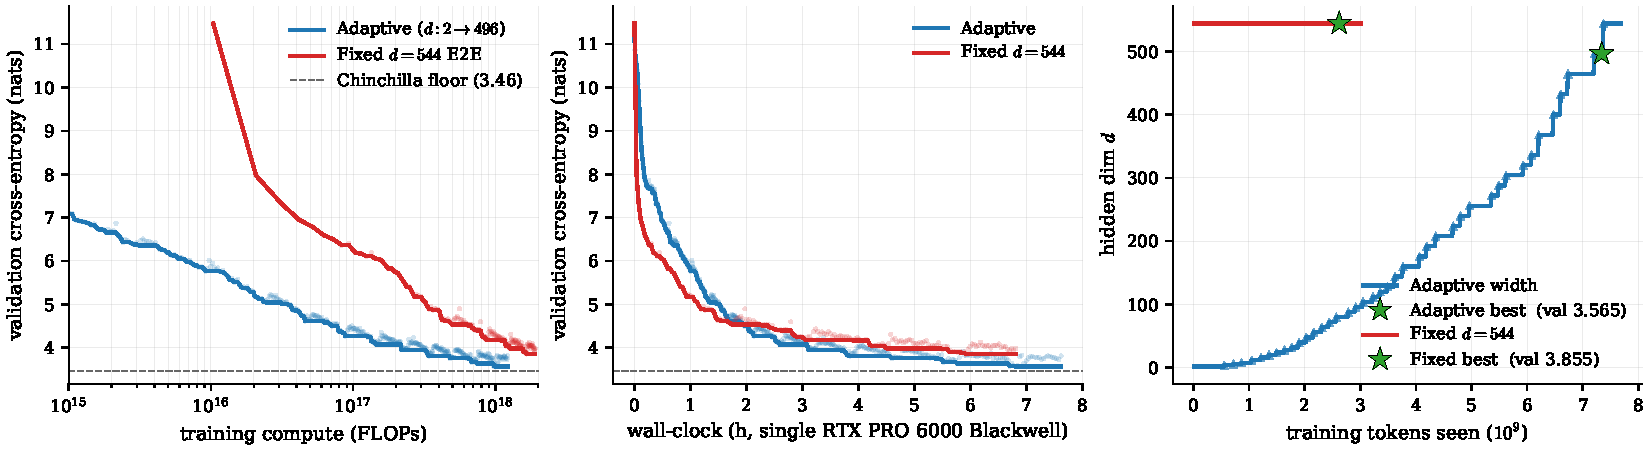
\includegraphics[width=\linewidth]{adapt_vs_e2e.pdf}
\caption{Adaptive (start $d{=}2$, grow to $d{=}544$, blue) vs fixed
$d{=}544$ E2E from scratch (red).  Left: val CE vs FLOPs used (log
$x$).  Middle: val CE vs wall-clock (h).  Right: width $d$ over tokens
seen, with grow events as triangles and best checkpoints as stars.}
\label{fig:adapt-vs-e2e}
\end{figure}

\begin{figure}[h]
\centering
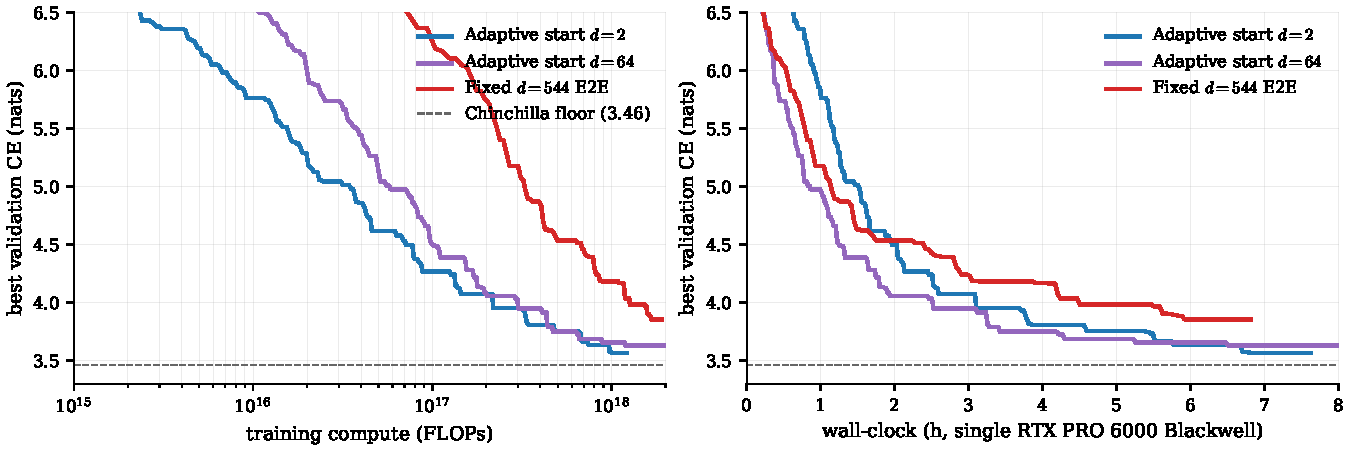
\includegraphics[width=0.85\linewidth]{startd_ablation.pdf}
\caption{Start-$d$ ablation: adaptive from $d{=}2$ (blue) and from
$d{=}64$ (purple), and fixed $d{=}544$ E2E (red), all with identical
training setup on the same GPU.  Starting from $d{=}2$ wins both
FLOPs-to-best and wall-clock-to-best; see \S\ref{sec:same-d} for
analysis.}
\label{fig:startd}
\end{figure}

\begin{table}[h]
\centering
\caption{Best checkpoint summary.  Both runs were trained for the same
total wall-clock $6.81$h on the same GPU; ``wall to best'' is the wall
at which each run's best eval occurred.  The adaptive run's best is
its last eval (still descending when stopped); the fixed-$d$ baseline
plateaus and does not improve over the remaining $\sim 1$h of wall.}
\begin{tabular}{lrrr}
\toprule
 & best val CE & FLOPs to best & wall to best \\
\midrule
Adaptive (d=2$\to$496)         & \textbf{3.565} & $1.00 \times 10^{18}$ & $6.81$ h \\
Fixed $d{=}544$ (matched wall) & 3.855          & $1.66 \times 10^{18}$ & $5.92$ h \\
\bottomrule
\end{tabular}
\end{table}

At matched wall-clock the adaptive run wins by $-0.29$ val CE while
also using $\approx 1.7{\times}$ fewer FLOPs to reach its best.  Best
adaptive checkpoint: \textbf{val CE $=3.565$ at $d{=}496$}, reached
after $6.81$ wall-hours.  We make no claim about behavior at much
higher FLOP; the adaptive trajectory plateaus near the Chinchilla
floor predicted for our $(N, D)$, so we do not expect further
substantial descent without more data.  The full per-$d$ trajectory
is in Appendix~\ref{app:trajectory}.

\subsection{Start-$d$ ablation}
\label{sec:startd-ablation}

We rerun the adaptive trajectory with starting width $d{=}64$
(skipping $d \in [2, 32]$) to test whether the small-$d$ phase is
``wasted compute''.  Both adaptive runs share data stream, tokenizer,
context length, eval batch, optimizer, learning rate, grad clip, and
$d_{\text{head}}$ schedule; the only change is the starting $d$.
Best checkpoints at matched wall-clock $6.81$h:

\begin{center}
\begin{tabular}{lrrr}
\toprule
 & best val CE & FLOPs to best & wall to best \\
\midrule
Adaptive start $d{=}2$    & \textbf{3.565} & $1.00 \times 10^{18}$ & $6.81$ h \\
Adaptive start $d{=}64$   & 3.628          & $1.20 \times 10^{18}$ & $6.51$ h \\
Fixed $d{=}544$ E2E       & 3.855          & $1.66 \times 10^{18}$ & $5.92$ h \\
\bottomrule
\end{tabular}
\end{center}

Starting from $d{=}2$ wins both metrics.  This is initially
surprising --- the small-$d$ phase has poor GPU utilization (matmuls
fall below the kernel-launch break-even) and feels like wasted
compute.  Two effects explain why it still wins.

(i) \emph{Chinchilla-optimal $N(D) \approx D/20$.}  At low token
counts $D$ the optimal model size is itself small; growing from
$d{=}2$ stays near the per-FLOP-loss frontier throughout, while
$d{=}64$ from scratch is over-parameterised for its early $D$ and
pays a flat warmup cost before benefiting from its capacity.

(ii) \emph{Width-dimension curriculum.}  PAVING-style grow with
zero-pad init means each dimension's training time depends on
\emph{when} it was added: dims $0$--$1$ are trained for the entire
run, dims $400$--$496$ only for the final few thousand steps.
Starting from $d{=}2$ gives the first dims an order of magnitude
more updates than starting from $d{=}64$ would, and these
well-trained early dims serve as a strong basis on top of which
later dims are stacked.  Cold-starting all $64$ dimensions
simultaneously skips this curriculum.

The wall-time penalty of the small-$d$ phase is real but is more
than offset by these two effects in our setup.  We have not searched
for the wall-optimal start $d$; we expect a sweet spot somewhere
between $2$ and $64$ for hardware where kernel-launch overhead
dominates more than ours.

\subsection{Width Detach --- Numerical Verification}

We rerun the proof script \texttt{proofs/width\_detach.py} at
$d \in \{64, 128, 256, 512\}$ and $g \in \{0.1, 0.05, 0.01\}$.
Empirical gradient distances scale as predicted ($O(g^2)$); typical
errors are $10^{-5}$ to $10^{-7}$, several orders of magnitude below
the gradient norm.  See the script output for the exact per-$d$ /
per-$g$ values.

\subsection{Future ablations}
\label{sec:ablations}

\begin{itemize}
\item Net2Net-style clone-grow init in place of zero-pad, to test
  whether the lower $d_{\text{eff}}{=}0.5$ observed mid-trajectory is
  the dominant inefficiency.
\item A finer start-$d$ sweep around the wall-optimal sweet spot
  ($d \in \{8, 16, 32, 48\}$) to identify the kernel-launch
  break-even on our hardware.
\end{itemize}

\section{Limitations}
\label{sec:limitations}

\paragraph{Data-bound by Chinchilla.}
With 2.9B training tokens our $(N, D)$ falls in the data-bound regime
of Hoffmann \emph{et al.}'s scaling law: at $d{=}544$ ($N \approx
105$M, $20$ tokens/param) the predicted loss floor is $\approx 3.46$,
and our best $3.565$ is within $0.10$ of that floor.  Further val
descent requires more training tokens, not more parameters.

\paragraph{Stability past $d \approx 66$ (early diagnostic).}
An earlier configuration of this run (\texttt{bf16+AdamW8bit},
$\eta=3{\times}10^{-4}$, fixed $d_{\text{head}}{=}2$) stalled near
$d{=}66$: beyond the best checkpoint there, val drifted upward by
$\sim 0.2$ over several thousand steps.  Diagnostics resumed from
the $d=46$ checkpoint identified two contributors:
\begin{itemize}
\item \textbf{Mixed-precision optimizer state.}
  Holding everything else fixed and switching the forward to
  \texttt{fp32} with \texttt{torch.optim.AdamW} (no \texttt{bf16}
  autocast, no \texttt{AdamW8bit}) removes the post-best drift entirely:
  the same checkpoint that drifted $5.19 \to 5.47$ in
  \texttt{bf16+AdamW8bit} instead descends to $5.10$.  We attribute the
  drift to systematic bias in the 8-bit optimizer second-moment state
  accumulating over tens of thousands of steps in a direction that's
  uncorrelated with the gradient signal.
\item \textbf{Learning rate is too high for our scale.}
  Even in \texttt{fp32}, $\mathrm{LR}=3{\times}10^{-4}$ starts to drift
  at $d \approx 46$: the per-step loss change $\eta \,\|g\|_1$ exceeds
  the eval-batch noise floor, and noise compounds into a slow upward
  walk.  The bound
  $\eta_{\max} = \sigma_{\text{eval}}/\sqrt{N}$ from
  \S\ref{sec:lr-bound} predicts this transition near $d \approx 40$
  for our parameter count.  Dropping to $\mathrm{LR}/2$
  ($\eta = 1.5\!\times\!10^{-4}$) restores monotone descent past
  $d=46$ in the corrected run; the LR sweep at fixed $d=46$
  (Appendix~\ref{app:lr-sweep}) gives the same picture.
\item \textbf{Grow events spaced at the recovery floor.}
  Each grow has a one-time mean/var shock from the ActiveLayerNorm
  $d_{\text{active}}$ change, and the new attention heads' gates take
  several thousand steps to fill in; with grow events spaced
  ${\sim}4000$ steps apart at the post-$d=40$ band the recoveries do
  not stack cleanly.  The divergence guard keeps this from spiralling
  ---trajectories plateau rather than diverge--- but they plateau
  \emph{above} the best.
\end{itemize}
With \texttt{fp32} optimizer and $\mathrm{LR}/2$ applied above
$d \approx 40$, the run reaches $5.04$ at $d{=}46$ and continues
descending; manual LR step-downs to $\mathrm{LR}/4$ at $d{=}50$ carry
the trajectory through $d{=}66$ and beyond.  A second constraint
appears past $d{=}66$: with $d_{\text{head}}{=}2$ fixed, the per-head
attention score tensor has shape $B \times (d/2) \times T^2$, so VRAM
scales linearly with $d$ on top of the usual model-size cost; at
$d{=}66$ this already exhausts $94\,\text{GB}$ in pure \texttt{fp32}.
The main run uses the stepped $d_{\text{head}}(d) \in
\{2,4,8,16,32\}$ from \S\ref{sec:dhead} so the number of heads is
bounded above by $\sim 16$ throughout, eliminating the linear-in-$d$
attention memory term.

\paragraph{Not vs SOTA, not at frontier scale.}
This is a single-GPU run with 22 layers, $\le 105$M parameters at
peak, on $2.9$B tokens.  We make no claim about SOTA on FineWeb-Edu;
the comparison is exclusively against an E2E run of the same
architecture at the same final width under matched wall-clock.

\section{Related Work and Discussion}

We do not catalog progressive training broadly; the closest line is
Net2Net function-preserving width growth and stage-wise training of
mixture-of-depths or progressive-stack transformers.  PAVING differs
by (i) deriving the per-FLOP efficiency upper bound directly from the
weight-tied $K$-block construction and (ii) providing an exact
width-elastic LayerNorm.  Our contribution is empirical: a
single-run demonstration that the prediction holds at the
$10^{18}$-FLOP scale on real text data (FineWeb-Edu, $2.9$B tokens,
22 layers, $d$ grown from $2$ to $544$), with a schedule that
requires no hand-tuned thresholds.

The natural follow-up is more training tokens (the current run is
within $0.10$ of the Chinchilla floor for our $(N, D)$), and a clone-
or distribution-extending grow init in place of zero-pad to lift the
mid-trajectory $d_{\text{eff}}{=}0.5$ ceiling we observe.

\bibliographystyle{tmlr}
\begin{thebibliography}{1}

\bibitem{paving} PAVING: weight-tied $K$-block elasticity, theorems and proofs.
Zenodo, DOI \href{https://doi.org/10.5281/zenodo.19454889}{10.5281/zenodo.19454889}.

\end{thebibliography}

\appendix

\section{Schedule of grows in the main run}
\label{app:trajectory}
See \texttt{paper/RESULTS.md} for the per-$d$ best-val table.  In
summary, the main run touches $d \in \{2, 4, 6, 8, \ldots, 64, 72,
80, \ldots, 256, 272, 288, \ldots, 496, 544\}$, growing by the
$d_{\text{head}}$-aware rule of \S\ref{sec:asymmetric-init}, and
reaches its best val $3.565$ at $d{=}496$ after $6.81$ wall-hours.

\section{LR and precision sweep at fixed $d=46$}
\label{app:lr-sweep}
Resumed from the main run's $d=46$ checkpoint (step $115\,000$,
val~$5.19$), no further grow events allowed, for an additional
$20\,000$ steps.  $N=3.2\!\times\!10^{6}$ parameters at this width.

\paragraph{LR sweep (\texttt{bf16+AdamW8bit}, unchanged precision).}
\begin{center}
\begin{tabular}{rrr l}
\toprule
$\eta/\eta_0$ & $\eta$ & best val & behavior \\
\midrule
$1$       & $3{\times}10^{-4}$  & 5.19 & drifts up to 5.47 then plateaus \\
$1/2$     & $1.5{\times}10^{-4}$& \textbf{5.03} & stable, monotone descent \\
$1/3$     & $1{\times}10^{-4}$  & 5.19 & spikes to 8+ twice in 20k steps \\
$1/10$    & $3{\times}10^{-5}$  & 5.08 & stable \\
$1/30$    & $1{\times}10^{-5}$  & 5.14 & stable, slow \\
\bottomrule
\end{tabular}
\end{center}

\paragraph{Precision toggle ($\eta = 3{\times}10^{-4}$, same checkpoint).}
\begin{center}
\begin{tabular}{l r l}
\toprule
precision & best val & behavior \\
\midrule
\texttt{bf16} + \texttt{AdamW8bit} & 5.19 & drifts up to 5.47 \\
\texttt{fp32} + \texttt{torch.optim.AdamW} & \textbf{5.10} & monotone descent \\
\bottomrule
\end{tabular}
\end{center}

The sweet spot in the LR sweep is $\eta_0/2$ (best val $5.03$); see
\S\ref{sec:lr-bound} for the $\sqrt{N}$-scaling argument and the
gap from the worst-case bound.  In the precision toggle, both rows
use the same $\eta = 3{\times}10^{-4}$; the only change is the
optimizer / forward precision, and that change alone removes the
drift.

\section{Hyperparameters}
\label{app:hyperparams}
See \S\ref{sec:method} and the schedule constants in
\texttt{adaptive\_growth.py}.

\section{Width Detach numerical verification details}
See \texttt{proofs/width\_detach.py} in the same repository for the proof
script and its numerical verification.

\end{document}
